\documentclass[12pt]{elsarticle}
\usepackage{newtxtext}
\usepackage[margin=1in]{geometry}
%\pagestyle{empty}
\usepackage{natbib}
\bibliographystyle{unsrt}
\usepackage{color}
\usepackage{amsmath}
\usepackage{hyperref}
\usepackage{wrapfig}
\usepackage{titlesec}
\usepackage{colortbl}
\titleformat{\section}[runin]{\normalfont\bfseries}{\thesection.}{3pt}{}


\begin{document}

\begin{center} \textbf{PROJECT NARRATIVE} \end{center}

%
\section{Goals and objectives} [note the RFP does not require a section for goals and objectives, but I believe a summary upfront will increase readability of the proposal]
\subsection{Goals}
\begin{enumerate}
\item
\item
\item
\end{enumerate}

\subsection{Objectives}
\begin{enumerate}
\item Synthesize methods and datasets for fish passage prioritization for all counties, and any other entities using prioritization indices, within the Washington state injunction area.
\item Generate a geospatial dataset of current usual and accustomed fishing areas for tribal nations in Western Washington.
\item Generate predicted cost estimates for all barriers to fish passage within the Washington state injunction area. 
\end{enumerate}

\clearpage
%
\section{Background}
\subsection{Fish passage in Washington state}


\begin{wrapfigure}{r}{10cm}
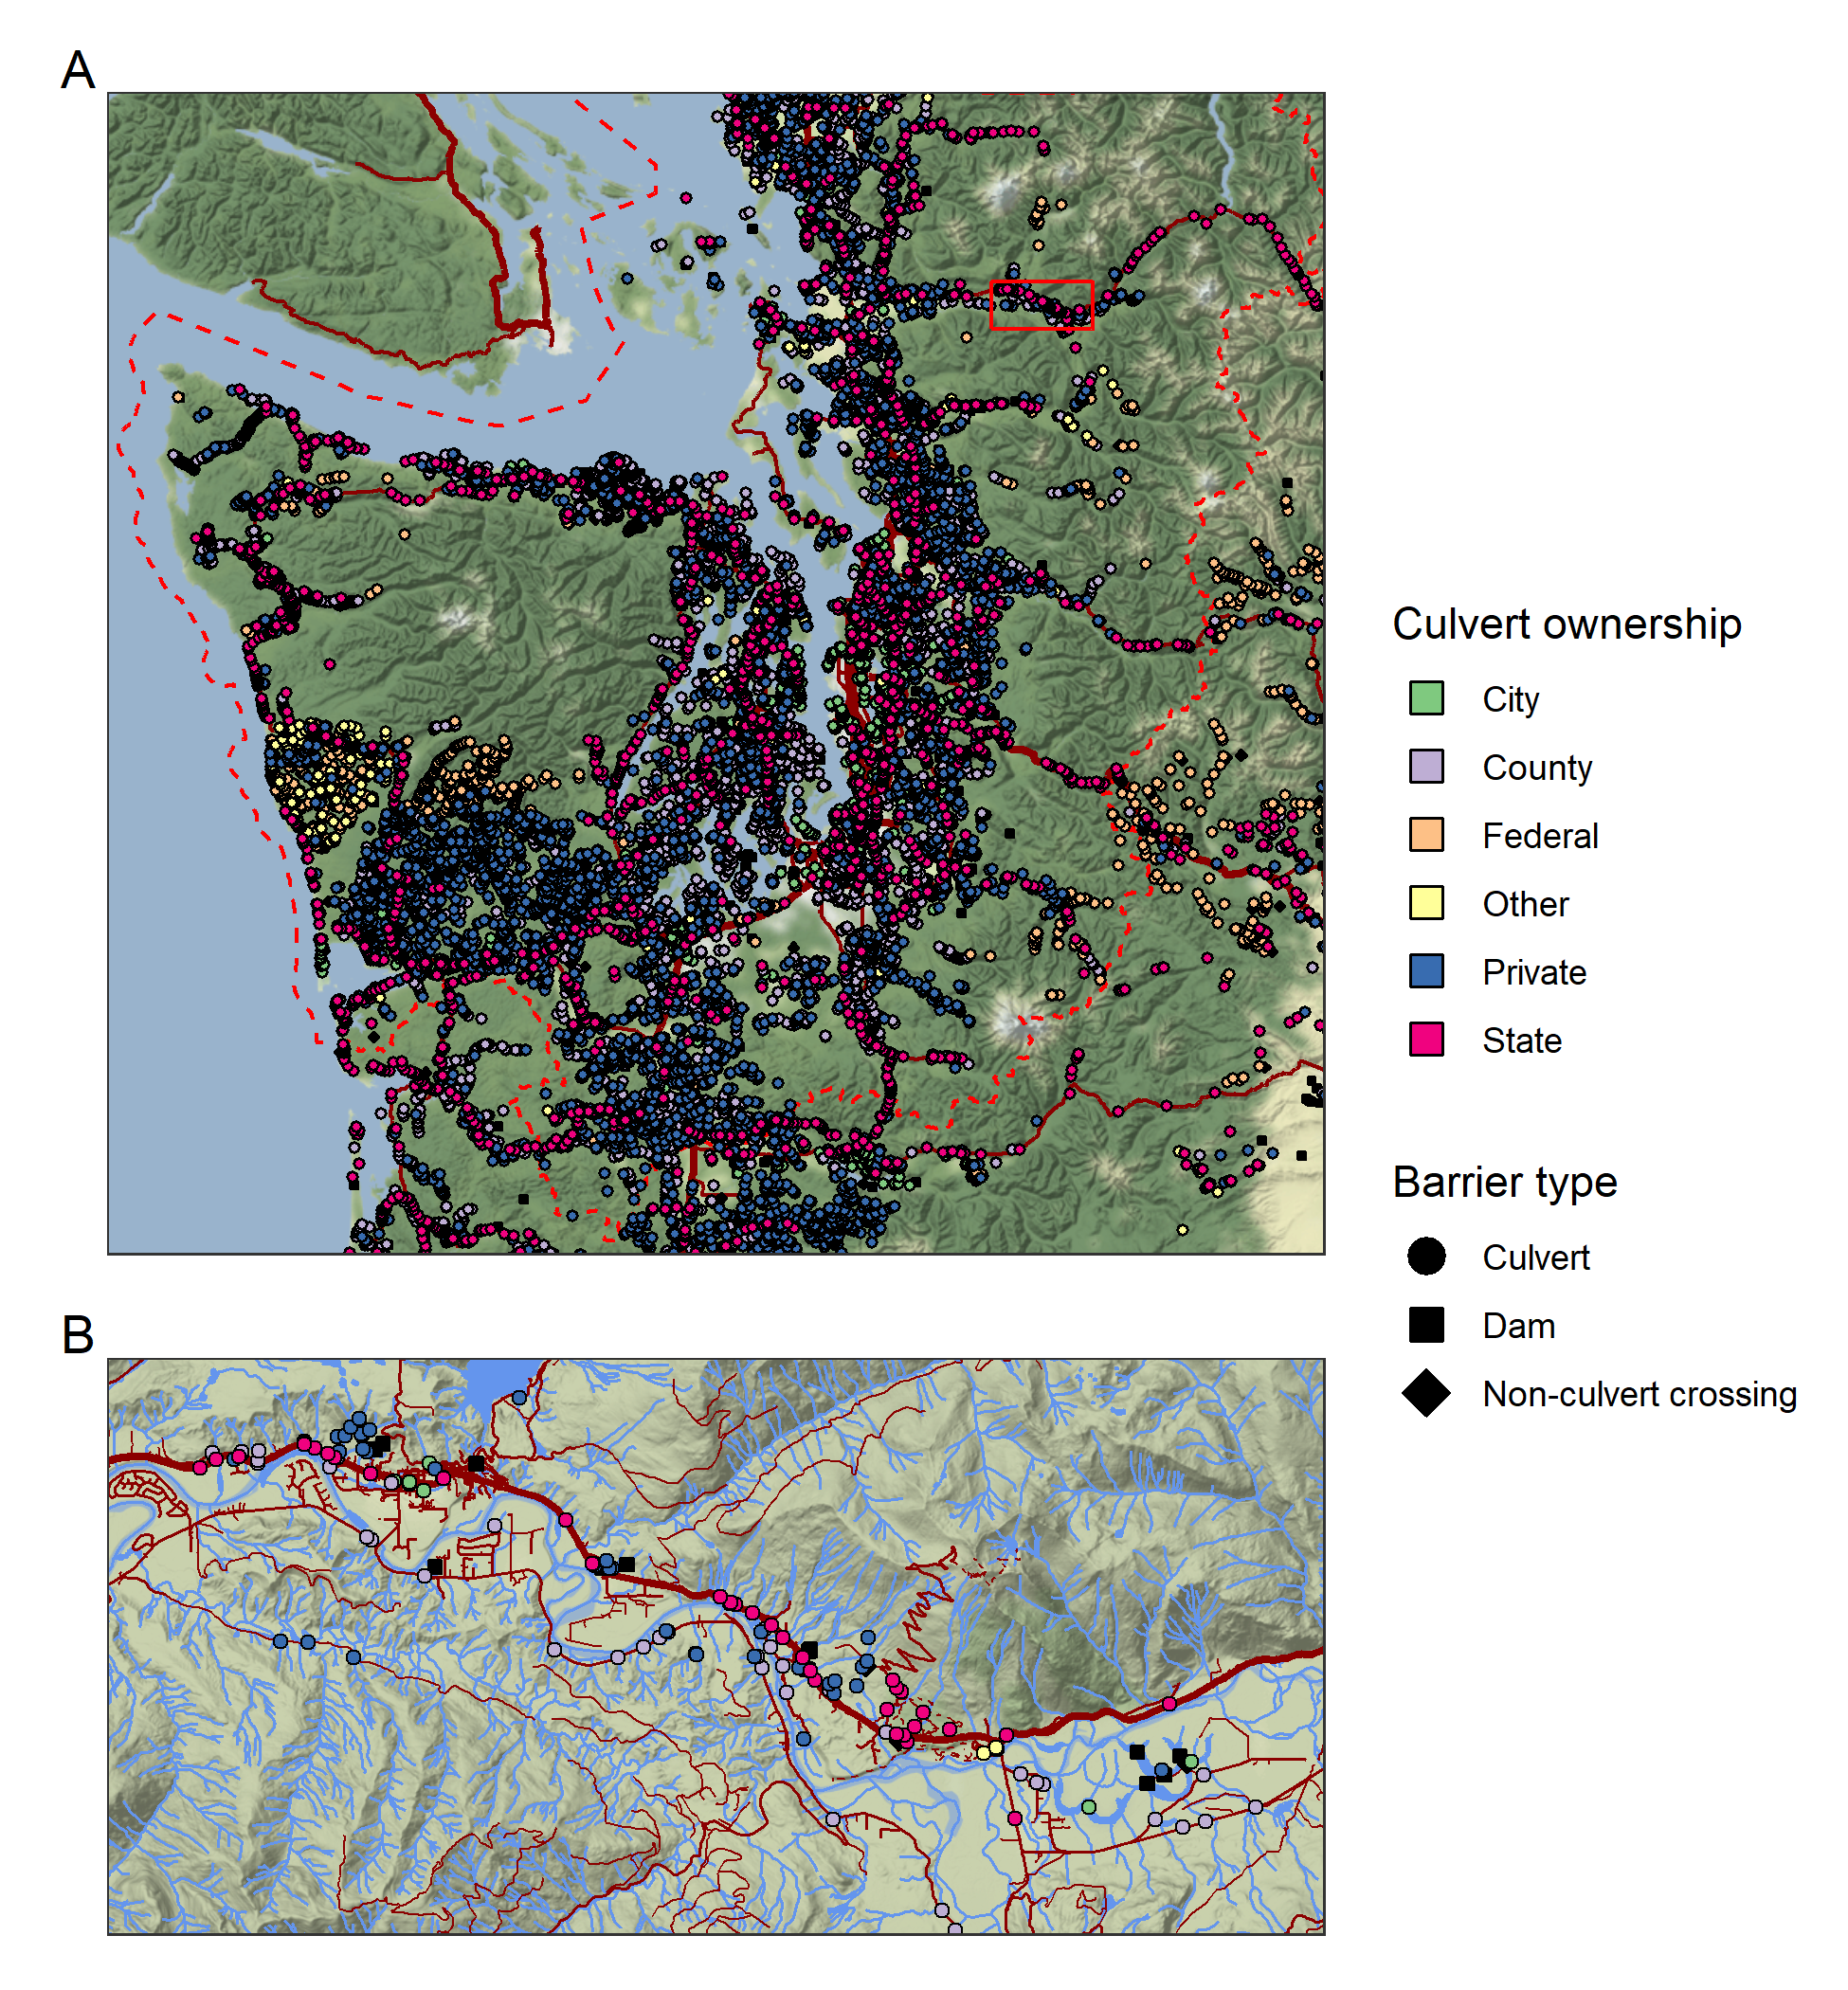
\includegraphics[width=10cm]{figures/fig_mapconcrete.png}
\caption{Barriers to fish passage in the WDNR XXXX database by ownership type. The small-scale map shows the entire Washington state injunction area (red dotted line) and the large-scale map shows barriers to fish passage for all ownership types for XXXXX.\label{fig:barrierMap}}
\end{wrapfigure}%



 In 2001, Washington State was sued by the United States Department of Justice on behalf of 21 Northwest tribes for violating treaty fishing rights. The plaintiff argued that state-owned culverts are barriers to salmon and steelhead accessing historical upstream spawning habitat, violating the Stevens Treaties \citep{hickey2018highway}. The lawsuit resulted in a 2013 federal court injunction requiring the state remove barrier culverts under its jurisdiction by 2030. After nearly two decades of legal battles, in 2018, the U.S. Supreme Court ruled in favor of the tribes, upholding the 2013 federal injunction. 

As of 2020, the Washington State Department of Transportation (WSDOT), responsible for the vast majority of state-owned culverts within the case area, has corrected 87 injunction barrier culverts opening up an estimated 383.3 miles of habitat at a cost of over \$159 million. Since the ruling, WSDOT has replaced an average of 12.4 culverts per year, including 13 in 2020. To satisfy the federal injunction, the rate of culvert replacements must ramp up dramatically. 

Importantly, the 2013 injunction strictly applies to state-owned culverts whereas there exist an estimated 3,000 and 1,300 additional barrier culverts owned by counties and cities respectively, along with barrier culverts on private lands, often on the same streams as state-owned culverts \citep{brown2019coming}. Figure~\ref{fig:barrierMap} shows blockages to fish passage recorded in the Washington Department of Natural Resources (WDNR) database for each of 6 ownership types: cities, counties, federal, private, state, and other. There is heterogeneity within many of these ownership types in terms of goals, priorities, and resources for removing barriers to fish passage. For example, while some cities and counties are able to access the financial resources for fish passage projects, e.g.\ King county has used the surface water management fee to fund culvert restoration projects, other cities and counties do not have access to dedicated funding streams, primarily relying on grant funding.  

The Brian Abbott Fish Barrier Removal Board, established by the Washington State Legislature, to recommend priority projects to the Governor's Office and Legislature for funding, thereby promoting the coordinated and strategic removal of barriers to fish passage. In the 2021-2023 biennium, 87 ranked projects were recommended for funding at a total of \$61.3 million. Grant applicants include cities, counties, and non-profit organizations.

Currently WSDOT, the Brian Abbott Fish Barrier Removal Board, and cities and counties all \textcolor{red}{DESCRIBE THE PRIORITIZATION INDEX METHOD.}


\subsection{Optimization tools in fish passage}

While there is a rich academic literature applying optimization tools to fish passage (CITES), recently these tools have gained traction with resource managers. Here we highlight two such applications of optimization tools used in fish passage. 

In the fall of 2019 the California Fish Passage Forum announced the launch of a web-based user-friendly optimization DST called \href{https://fishpass.psmfc.org}{FISH\emph{Pass}} to guide strategic planning around fish passage barrier removal across the state. The development of FISH\emph{Pass} resulted from a collaborative effort between the California Fish Passage Forum, the National Fish Passage Program, the Pacific States Marine Fisheries Commission, and others and is based on the mixed integer linear programming optimization framework developed by \citet{o2005optimizing}. The adoption of FISH\emph{Pass} in California replaced rank and score methods with stated goals of improving objectivity in recommendations, providing a systematic framework to project selection given limited financial resources, and balanced multiple and possibly competing objectives and constraints. Currently, the California Fish Passage Forum is funding research that will apply the FISH\emph{Pass} tool to the Smith River watershed to learn about the performance of FISH\emph{Pass} and identify approaches and data inputs to strengthen the model.

%\href{https://www.cafishpassageforum.org/2020-projects}{Currently, the California Fish Passage Forum is funding research that will apply the FISH\emph{Pass} tool to the Smith River watershed to learn about the performance of FISH\emph{Pass} and identify approaches and data inputs to strengthen the model.}

A second application is \href{https://greatlakesconnectivity.org}{FishWerks} developed for the Great Lakes region as a collaboration between Cornell University and the University of Wisconsin. The FishWerks DST allows users to generate restoration plans including dam removal and barrier culvert restoration. \citet{moody2017pet} identify three necessary features for a DST to bring value to users. First, the underlying data must be dynamic and up-to-date. Second, maintenance must be made easy to ensure use, because organizations rarely have the resources including technical staff to support hosting and maintaining the DST beyond the initial project period. Third, due to a potential perceived black box nature of an optimization DST, the tool must offer significant improvements to the simpler planning methods to ensure adoption.

\subsection{Optimization for Washington fish passage}

%
\section{Approach}
\subsection{Cost model}
\subsection{Habitat model}
\subsection{Equity}
\subsection{Risk mitigation}

\begin{itemize}
\item Climate change projected to affect peak water flow during egg incubation, stream temperature during pre-spawning, and minimum flow during spawning \citet{battin2007projected} with greatest impacts in high-elevation streams with less barrier culverts. 
\end{itemize}

\subsection{Network configuration}
\subsection{Ownership}

\subsection{Optimization \label{sec:opt}}

\begin{wrapfigure}{r}{0.5\textwidth}
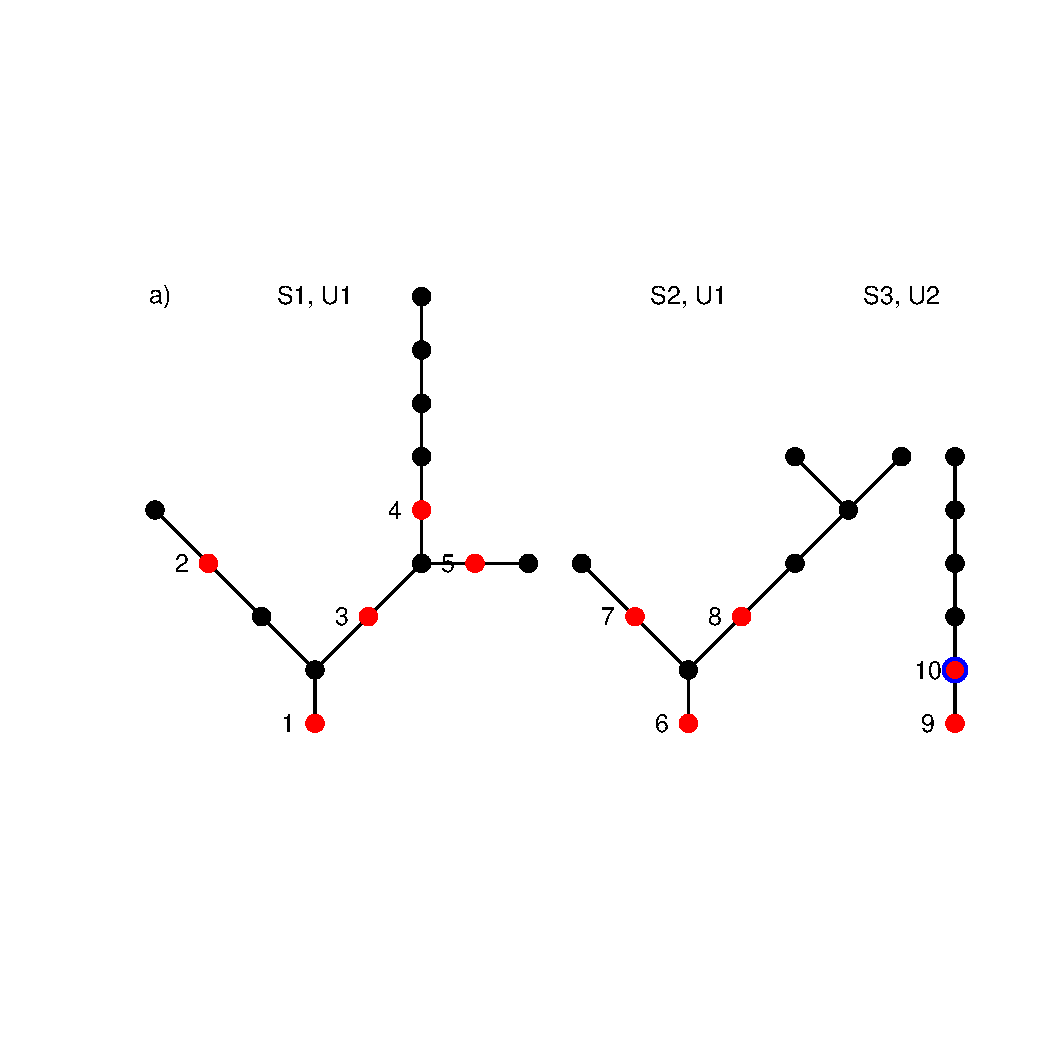
\includegraphics[width=0.48\textwidth]{figures/opt_s.pdf}
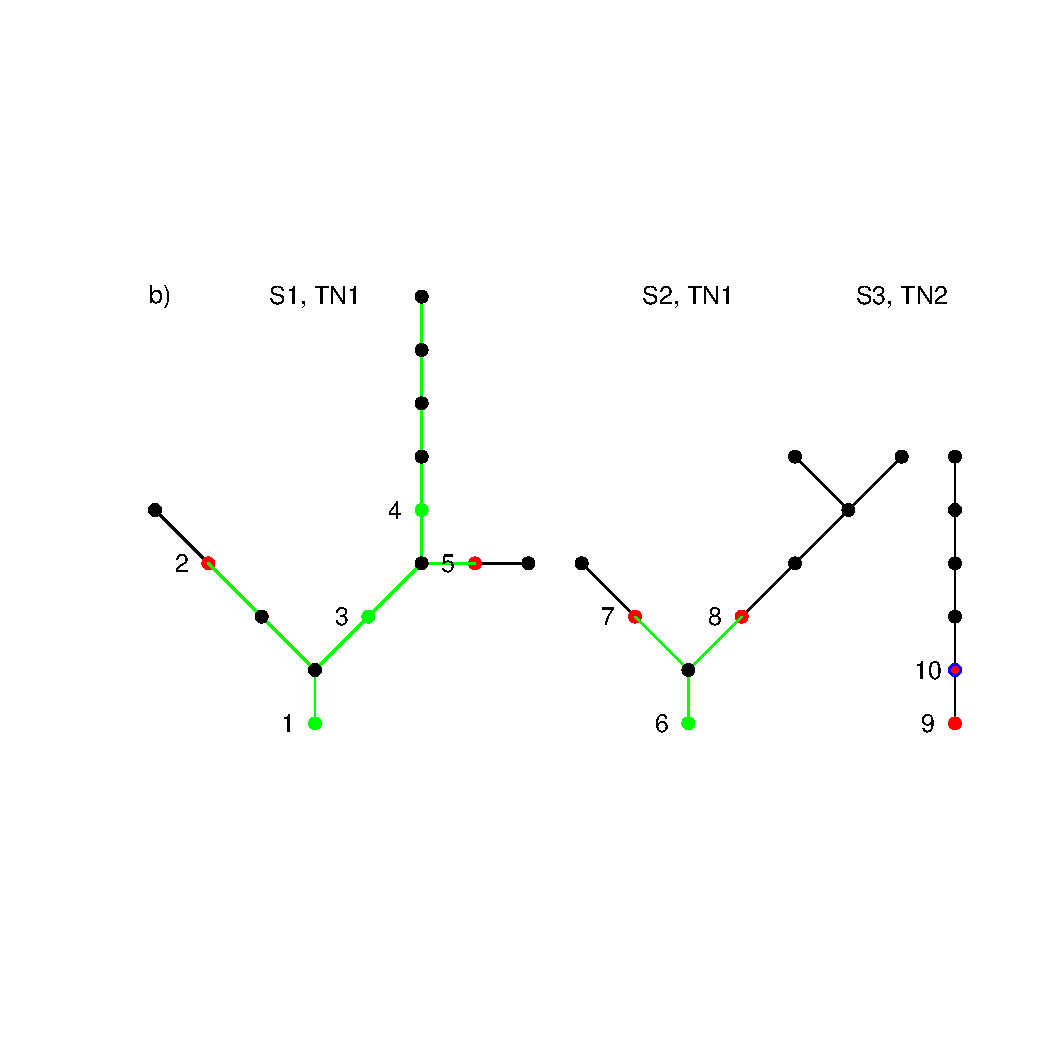
\includegraphics[width=0.48\textwidth]{figures/opt_h.pdf}
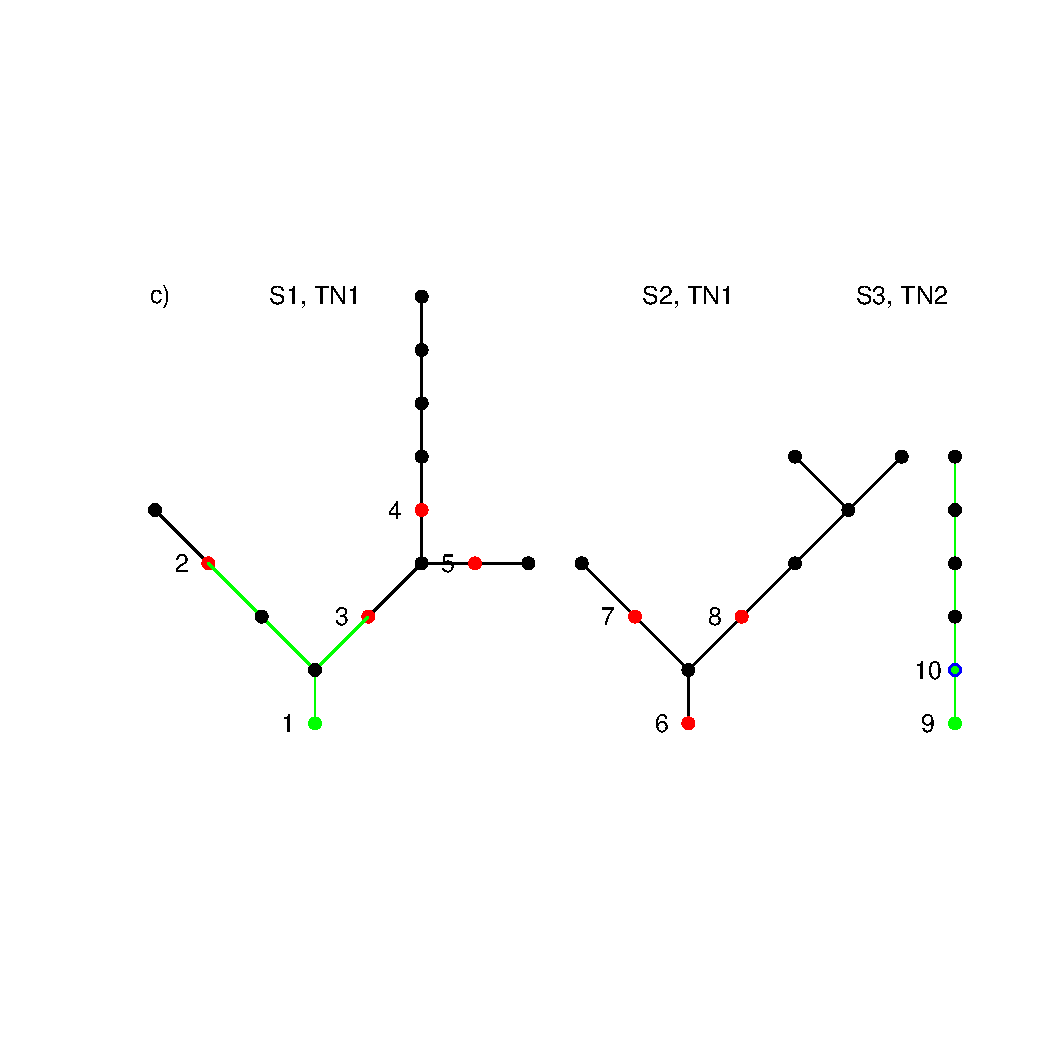
\includegraphics[width=0.48\textwidth]{figures/opt_e.pdf}
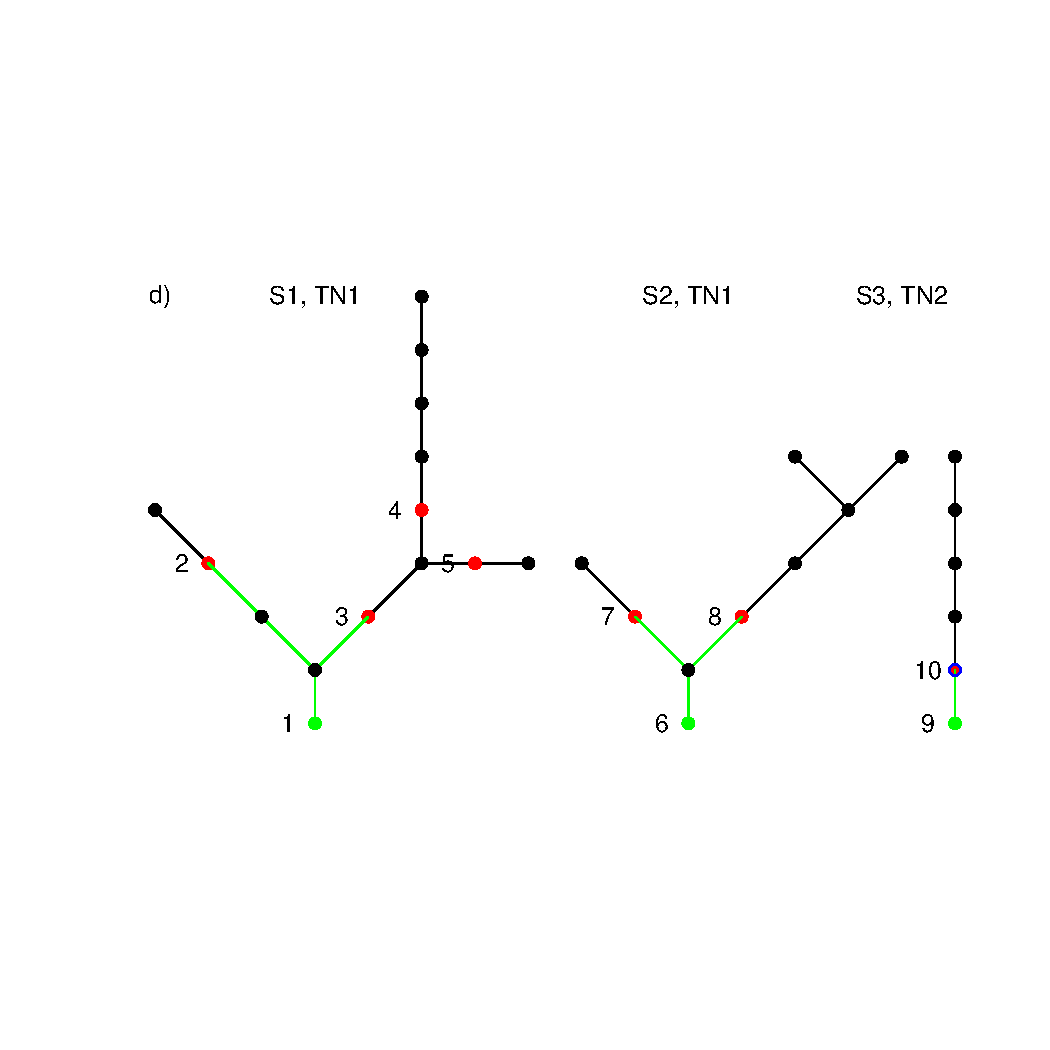
\includegraphics[width=0.48\textwidth]{figures/opt_d.pdf} 
\caption{Solutions to a scalarized multiobjective problem in a stylized system where there are 3 salmon stocks (S1-S3) and 2 tribal nations (TN1-TN2). \label{fig:opt}}
\end{wrapfigure}%


We will explore two alternative approaches to define cost-effective restoration plans that meet multiple planning goals (e.g.\ salmon habitat gains, equity considerations, and risk mitigation). Both approaches are considered ``a priori'' methods for multiobjective optimization because the decision maker must specify their preferences related to the various objectives prior to the optimization. 

In the first approach (i.e.\ linear scalarization), managers specify importance weights for each of the objectives and the weighted sum of the objectives is maximized. Weights are constrained to the interval [0, 1] and sum to one, e.g.\ a manager solely interested in habitat would set the habitat importance weight to 1 and all other weights to zero. The problem will also include a budget constraint, such that expenditures on barrier restoration are less than or equal to a fixed budget $B$, and a hydrography constraint such that habitat gains from restoring any one barrier cannot be realized if there exist any downstream barriers to fish passage. Figure~\ref{fig:opt} demonstrates solutions to this first optimization approach with a budget constraint of \$40. Panel (a) represents a model system with 10 barrier culverts (numbered red markers), 26 units of potential habitat (increments between two adjacent markers represent 1 unit of habitat), on 3 streams utilized by 3 salmon stocks (S1-S3), harvested by two tribal nations (TN1-2). Each of the culverts 1-9 costs \$10 to restore while culvert 10 costs \$20 to restore (and is outlined in blue).

Panel (b) represents the habitat-maximizing solution (the habitat weight is set to one and all other weights are set to zero) , with 14 units of habitat gained (11 on stream 1 and 3 on stream 2), but all of the benefits going to a single tribal nation. In the habitat-maximizing solution, the budget is exhausted by restoring 4 culverts for a total cost of \$40. Panel (c) represents the equity-maximizing approach (the equity weight is set to one and all other weights are set to zero), with 9 units of habitat restored (4 on stream 1 and 5 on stream 3). In this solution, the budget is also exhausted and the habitat gains are nearly evenly split across tribal nations (4 for Tribal Nation 1 and 5 for Tribal Nation 2). Finally, panel (d) represents the diversification-maximizing solution (the weight on diversifying habitat gains across salmon stocks is set to one and all other weights are set to zero), with a total of 8 units of habitat gained (4 on stream 1, 3 on stream 2, and 1 on stream 3) spread across the three salmon stocks. Interestingly, the budget is not exhausted in the diversification-maximizing solution as total expenditures for the 3 culverts restored is \$30. Whenever objective functions are defined by even allocations, e.g.\ across tribal nations or salmon stocks, the budget constraint may not hold.

In the second approach (i.e.\ $\epsilon-$constraint method), one objective function is maximized and lower bounds, $\epsilon$ parameters are provided for all remaining objectives. For example, the problem can be defined to maximize habitat gains subject to each tribal nation receiving some minimum fraction of the habitat gains or some minimum fraction of total expenditures, or a constraint such that habitat gains are distributed across some minimum number of salmon stocks.


%As an illustrative example of the first approach, suppose Lewis County wants to define a restoration plan (a package of culverts to be restored) that balances habitat increases for Chinook salmon in the injunction area with equity and risk mitigation. Further suppose Lewis County had a budget of B dollars to invest in the restoration plan and does not want to restore any culverts outside of its jurisdiction. Our framework would solve the following problem (blue text represents manager inputs):
%\begin{equation*}
%\substack{\text{\large max}}_{\boldsymbol{c}}\hspace{0.25in} \textcolor{blue}{w_1}\:\: \text{Chinook habitat metric} + \textcolor{blue}{w_2}\:\: \text{equity metric} + \textcolor{blue}{w_3}\:\: \text{risk mitigation metric},
%\end{equation*}
%\noindent subject to:  
%\begin{equation*}
%\text{total cost} \le \textcolor{blue}{B} 
%\end{equation*}
%\begin{equation*}
%\boldsymbol{c} \in \{\textcolor{blue}{\boldsymbol{c}_{lewis}}  \},
%\end{equation*}
%\begin{equation*}
%\text{hydrography}
%\end{equation*}
%
%where $\boldsymbol{c}$ are culverts included in the restoration plan, $\boldsymbol{c}_{lewis}$ are the subset of barrier culverts owned by Lewis county, B is total amount of funding that can be spent, and $w_1-w_3$ are the weights that managers place on each objective. The problem will be additionally constrained so that benefits from upstream culvert removal cannot be captured without first removing downstream blockages.
%
%As an illustrative example of the second approach, suppose Lewis County wants to define a restoration plan that maximizes habitat but 



\subsection{Role of team members and partners}
\textbf{PI Jardine} will serve as the lead administrator of the grant where administrative responsibilities include organizing meetings both internally and with the scientific advisory board to ensure the project is on track to deliver work products on time, tracking project performance, facilitating project design decisions, and supervising and mentoring the postdoctoral scholar and the Sea Grant Fellow.  PI Jardine will also provide technical assistance with optimization in R and developing the R Shiny app including providing template code for various optimization algorithms along with sensitivity analyses and model selection, and providing template code for the DST user app features.\\


%
\section{Engagement plan}
\subsection{Community collaborators} 

\begin{table}[h]
\caption{Anticipated Scientific Advisory Board \label{tab:sab}}
\centering
\begin{tabular}{lcc}\hline
 Name & Job Title & Affiliation  \\\hline
Jeff Dickison& Asstistant Natural Resources Director &  Squaxin Island Tribe\\
& & Natural Resource Center\\
\rowcolor[gray]{.9} Steve R Hinton &  Conservation Scientist&  Tulalip Tribes  \\
\rowcolor[gray]{.9}& &Treaty Rights \& Government Affairs\\\hline
\end{tabular}
\end{table}


\subsection{Target audiences}



\subsection{Engagement activities}

In the beginning of YR1, in the initial phase of the project, we will organize a series of workshops intended to uncover the objectives and challenges in culvert barrier replacement for key user groups including WSDOT, city and county governments, restoration agencies such as the Fish Barrier Removal Board, WDFW, and representatives from relevant tribal nations. The workshops will begin with a presentation of our proposed framework and online tool (described in Section~\ref{sec:summary}) as a straw-man proposal in order to generate discussion and elicit ideas on how to capture fundamental real-world priorities and constraints in barrier culvert removal. We will gather feedback during the workshops and through post-workshop surveys. Ideas coming from the initial series of workshops will be incorporated into our project to the extent possible given data and computational limitations, which will be made clear to workshop participants.

In a second phase, at the beginning of YR2, we will organize a second series of workshops to present preliminary results (e.g.\ tradeoffs between various objectives) and demonstrate the functionality of a preliminary working version of the online tool. This second series of workshops will demonstrate how feedback from the initial workshops was incorporated in our framework and tool and provide a more in-depth discussion of our data inputs to the tool, e.g.\ a demonstration of the quality of our cost estimates and a visual demonstration of our preliminary spatial definition of our equity metric. The second series of workshops will provide stakeholders with a final opportunity to guide key features of the framework and solicit feedback on the usability of the online DST.

Finally, at the end of YR2, we will host an interactive workshop to launch our finalized online tool letting stakeholders directly engage with the tool. In preparation for this workshop, we will develop a video tutorial that will present content from the DST user guide in a way that is accessible and engaging. The workshop will begin with a screening of the video tutorial. Then, we will engage participants with exercises that highlight the tradeoffs between various objectives, gains from coordination, and how alternative budget/funding scenarios (defined by budget levels and their distribution across time) impact the culvert restoration packages with the highest return on investment. Each workshop participant will be provided with a laptop computer to participate in the exercises. 

At each phase of our engagement plan we will rely on advice from our Scientific Advisory Board (Table~\ref{tab:sab}). Members of our Scientific Advisory Board will include individuals working directly in the area of barrier culvert restoration, individuals with a history of engaging with our key stakeholder groups, and individuals generating science relevant to our problem area. We are actively working to construct a Scientific Advisory Board that has representation from XXXX.

\subsection{Anticipated outcomes and evaluation}

We anticipate two major research outcomes. First, our research will form the basis of a student thesis, leading to a scientific publication, applying our underlying optimization model to answer important research questions including:

\begin{enumerate}
\item How can equity be accounted for in in fish passage problems? (Note, to our knowledge equity has not been accounted for in the fish passage prioritization literature.)
\item How can project risk be accounted for in fish passage problems? (Note, to our knowledge risk has not been accounted for in the fish passage prioritization literature.)
\item What are the gains in habitat, equity, and risk avoidance associated with coordination across actors (state agencies, local government, private landowners) and which of these multiple objectives is most affected by a lack of coordination across actors?
\item Where in Washington injunction area (sub-basins/watersheds) are culvert restoration plans associated with tradeoffs between potentially competing priorities (e.g., risk versus total habitat, equity versus total habitat), and where can "win-wins" occur (i.e., plans that meet multiple objectives without reducing others)?
\item How do the two optimization approaches, described in Section~\ref{sec:opt}, compare in terms of how solution stability and computational efficiency.
\end{enumerate}


Second, our project will produce publicly-available, well-documented, open-source prioritization DST for barrier culvert removal in the Washington injunction area. The DST can serve a coordinating function by providing a framework to evaluate restoration plans across various actors regardless of whether the restoration plan is one identified by our optimization framework. The DST can also support planning for cities and counties with limited access to data and quality cost estimates. Finally, the source code behind our open-source DST will be made widely available to users outside of the state of Washington to facilitate the adoption of and customization by a larger set of potential users. 


\clearpage
\large References\\
\normalsize
\bibliography{wsg}
\end{document}